\subsection{Nilai Eigen dan Vektor Eigen}
Salah satu konsep penting yang berkaitan dengan transformasi linear dan materi yang membuat UTS penulis "sedikit" di bawah rata-rata adalah nilai eigen (\textit{eigenvalue}) dan vektor eigen (\textit{eigenvector}). Misalkan sebuah matriks persegi $\mathbf{A} \in \mathbb{R}^{n \times n}$. Sebuah skalar $\lambda \in \mathbb{R}$ disebut nilai eigen dari $\mathbf{A}$, jika terdapat vektor tak-nol $\mathbf{x} \in \mathbb{R}^n$ sehingga
$$
A\mathbf{x} = \lambda \mathbf{x}
$$

Vektor tak-nol $\mathbf{v}$ yang memenuhi persamaan tersebut disebut \textit{vektor eigen} yang berkaitan dengan nilai eigen $\lambda$.

Secara geometris, vektor eigen adalah vektor yang arahnya dipertahankan oleh matriks transformasi linier $\mathbf{A}$. Transformasi hanya mengubah panjang vektor dengan faktor skalar $\lambda$ tanpa memutar arah vektor tersebut.

\begin{figure}[H]
    \centering
    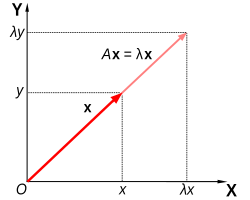
\includegraphics[width=0.3\textwidth]{assets/contoh-eigenvalue.png}
    \caption{\href{https://en.wikipedia.org/wiki/Eigenvalues_and_eigenvectors}{Interpretasi Geometris dari Nilai Eigen}}
    \label{fig:contoh-geometris-eigen}
\end{figure}

Persamaan $A \mathbf{x} = \lambda \mathbf{x}$ dapat ditulis kembali sebagai:
$$
(A - \lambda I) - \mathbf{x} = 0
$$

di mana $I$ adalah matriks identitas $n \times n$. Agar persamaan ini memiliki solusi tak-nol $\mathbf{x}$, matriks $A - \lambda I$ harus singular, sehingga
$$
    \det(A - \lambda I) = 0.
$$

Persamaan ini disebut persamaan karakteristik dari matriks $A$ dan akar-akarnya adalah nilai eigen $\lambda$ dari matriks tersebut. Untuk setiap $\lambda_i$ yang ditemukan, vektor eigen dapat dihitung dengan menyelesaikan $(A - \lambda_i I)\mathbf{x} = 0$.

Sebuah fakta penting dalam Aljabar Linier adalah bahwa matriks simetris memiliki sifat spektral yang sangat baik. Jika $A \in \mathbb{R}^{n \times n}$ adalah matriks simetris, maka:

\begin{IEEEitemize}
    \item Semua nilai eigen $\lambda_i$ dari $A$ adalah bilangan real.
    \item Vektor-vektor eigen yang berkaitan dengan nilai eigen yang berbeda saling ortogonal.
    \item Matriks $A$ dapat didiagonalisasi menggunakan matriks orthogonal, yaitu
    $$
        A = Q \Lambda Q^T,
    $$
    di mana $Q$ adalah matriks orthogonal yang kolom-kolomnya terdiri dari vektor-vektor eigen yang sudah dinormalisasi, dan $\Lambda$ adalah matriks diagonal yang berisi nilai-nilai eigen $\lambda_1, \lambda_2, \ldots, \lambda_n$ pada diagonal utamanya.
\end{IEEEitemize}
